\section{Технологическая часть}

В данной части рассматривается выбор средств реализации, описывается структура программы и приводится интерфейс программного обеспечения.

\subsection{Средства реализации}

В качестве языка программирования для разработки программного обеспечения был выбран язык программирования C++ \cite{cpp}. Данный выбор обусловлен следующими факторами:

\begin{itemize}
	\item C++ обладает высокой вычислительной производительностью, что очень важно для выполнения поставленной задачи;
	\item Данный язык изучался в рамках учебной программы.
\end{itemize}

В качестве среды разработки был выбран QtCreator \cite{qtcreator}. Он имеет инструменты для удобной разработки программ с использованием выбранного фреймворка для графического интерфейса Qt \cite{qt}.

\subsection{Структура программы}

На рисунке \ref{img:uml} представлена схема разработанных классов программы.

\img{150mm}{uml}{Структура классов программы}

Основные классы разработанной программы:

\begin{itemize}
	\item Object --- базовый класс объекта;
	\item Lens --- класс линзы;
	\item Light --- класс источника света;
	\item PolyObject --- класс полигонального объекта;
	\item Sphere --- класс сферы;
	\item Camera --- класс камеры;
	\item Tri --- класс, представляющий полигон (треугольник);
	\item Material --- класс, представляющий материал объекта;
	\item Visitor --- базовый класс для реализации паттерна \textit{Посетитель};
	\item IntersectVisitor --- класс паттерна \textit{Посетитель} для нахождения пересечения луча с объектами;
	\item Scene --- класс сцены;
	\item Tracer --- класс, содержащий алгоритмы трассировки лучей;
	\item MeasureWorker --- класс для управления замерами;
	\item RenderWorker --- класс для управления отрисовкой изображения;
	\item ObjectAddUiController --- класс для управления виджетами добавления объекта;
	\item ObjectDeleteUiController --- класс для управления виджетами удаления объекта;
	\item MainWindow --- класс главного виджета окна.
\end{itemize}

\clearpage

\subsection{Реализация алгоритмов}

Фрагменты реализации алгоритма представлены на листингах:

\begin{itemize}
	\item листинг \ref{lst:render_pixmap} --- основная, <<высокоуровневая>> функция отрисовки сцены;
	\item листинг \ref{lst:trace_ray} --- функция трассировки луча, используется для получения цвета пикселя изображения;
	\item листинг \ref{lst:closest_intersection} --- функция нахождения ближайшего пересечения луча с объектами сцены;
	\item листинг \ref{lst:compute_color} --- функция для рассчета цвета объекта с учетом освещения в точке пересечения с лучем;
	\item листинг \ref{lst:compute_refact} --- функция определения направления преломленного луча.
\end{itemize}

\begin{lstlisting}[label=lst:render_pixmap,caption=Функция отрисовки сцены на изображении]
void render_pixmap(const Scene& scene, QPixmap& pix)
{
	const auto& cam = scene.cam;
	QMatrix4x4 cam_rot, cam_rot_x, cam_rot_y, cam_rot_z;
	cam_rot_x.setToIdentity();
	cam_rot_x.rotate(cam.rot.x(), 1, 0, 0);
	cam_rot_y.setToIdentity();
	cam_rot_y.rotate(cam.rot.y(), 0, 1, 0);
	cam_rot_z.setToIdentity();
	cam_rot_z.rotate(cam.rot.z(), 0, 0, 1);
	cam_rot = cam_rot_z * cam_rot_y * cam_rot_x;
	QPainter paint{&pix};
	int height = pix.height();
	int width = pix.width();
	int rendered_pixels = 0;
	for (int y = 0; y < height; y++)
	{
		for (int x = 0; x < width; x++)
		{
			if (should_stop)
				return;
			QVector3D viewport_point = cam.get_viewport_point(x - width / 2, -y + height / 2, width, height);
			QVector3D direction = viewport_point - cam.pos;
			direction = cam_rot.mapVector(direction);		
			QColor col = Tracer::trace_ray(scene.objects, scene.lights, cam.pos, cam.pos + direction, 1, Vars::far_distance);
			paint.setPen(QPen{QColor{col}});
			paint.drawPoint(x, y);
			++rendered_pixels;
			if (rendered_pixels % 100 == 0)
				emit rendering_progress(rendered_pixels);
		}
	}
}
\end{lstlisting}


\begin{lstlisting}[label=lst:trace_ray,caption=Функция испускания луча]
QColor trace_ray(const QList<Object*>& objects, const QList<Light*>& lights, const QVector3D& beg, const QVector3D& end, double t_min, double t_max) {
	auto [closest_object, intersection_point, norm] = Tracer::closest_intersection_with_norm(objects, beg, end, t_min, t_max);
	if (closest_object == nullptr)
	return Vars::bg_color;
	QColor result_color{};
	const Material& m = closest_object->get_material();
	norm.normalize();
	result_color = Tracer::compute_color_with_lights(objects, lights, intersection_point, norm, (end - beg) * -1, m.spec_factor, m.dif_factor, m.color);
	if (m.refact_factor > 0) {
		QVector3D refact_dir = Tracer::compute_refact_direction(end - beg, norm, m.refact_factor);
		refact_dir.normalize();
		auto refact_color = Tracer::trace_ray(objects, lights, intersection_point, intersection_point + refact_dir * Vars::small_distance, t_min, t_max);
		result_color = colorSum(result_color, refact_color);
	}
	return result_color;
}
\end{lstlisting}


\begin{lstlisting}[label=lst:closest_intersection,caption=Функция нахождения пересечения луча с объектом сцены]
std::tuple<Object*, QVector3D, QVector3D>
closest_intersection_with_norm(const QList<Object*>& objects, const QVector3D& beg, const QVector3D& end, qreal t_min, qreal t_max)
{
	qreal closest_t = Vars::far_distance;
	Object* closest_obj = nullptr;
	QVector3D intersection_point, norm;
	IntersectVisitor v{};
	v.beg = beg;
	v.end = end;
	v.t_min = t_min;
	v.t_max = t_max;
	for (const auto& obj : objects) {
		if (should_stop)
		break;
		obj->accept(&v);
		if (!v.intersects) 
		continue;
		if (v.t_intersect < closest_t) {
			closest_t = v.t_intersect;
			closest_obj = obj;
			intersection_point = v.intersection_point;
			norm = v.norm;
		}
	}
	return {closest_obj, intersection_point, norm};
}
\end{lstlisting}


\begin{lstlisting}[label=lst:compute_color,caption=Функция рассчета цвета объекта в точке с учетом освещения]
QColor compute_color_with_lights(const QList<Object*>& objects, const QList<Light*>& lights, const QVector3D& point, const QVector3D& norm, const QVector3D& v, qreal s, qreal dif, QColor obj_color) {
	QColor result_color{};
	for (const auto& li : lights) {
		if (should_stop)
		break;
		switch (li->type)
		{
			case LightType::AMBIENT: {
				result_color = colorSum(result_color, colorMul(colorMul(obj_color, li->color), li->intensity));
				break;
			}
			case LightType::DIRECTIONAL:
			case LightType::POINT: {
				QVector3D l;
				double t_max;
				if (li->type == LightType::POINT) {
					l = li->position - point;
					t_max = 1;
				} else {
					l = li->direction;
					t_max = Vars::far_distance;
				}
				if (Vars::enable_shadows) {
					auto [shadow_object, shadow_intersection_point, shadow_norm] =
					Tracer::closest_intersection_with_norm(
					objects, point, point + l, 1e-3, t_max);
					if (shadow_object != nullptr) 
					continue;
				}
				double n_dot_l = QVector3D::dotProduct(norm, l);
				if (n_dot_l > 0) 
				result_color = colorSum(result_color, cmul(cmul(obj_color, li->color), ((li->intensity * n_dot_l / (norm.length() * l.length())) * dif)));
				if (s >= 0) {
					QVector3D r = (norm * 2 * QVector3D::dotProduct(norm, l)) - l;
					double r_dot_v = QVector3D::dotProduct(r, v);
					if (r_dot_v > 0) 
					result_color = csum(result_color, cmul(cmul(obj_color, li->color), (li->intensity * pow(r_dot_v / (r.length() * v.length()), s))));
				}
				break;
			}
			default:
			break;
		}
	}
	return result_color;
}
\end{lstlisting}


\begin{lstlisting}[label=lst:compute_refact,caption=Функция направления преломленного луча]
QVector3D compute_refact_direction(QVector3D direction, QVector3D norm, double refact_index) {
	direction.normalize();
	double eta = 1.0 / refact_index;
	double cos_theta = -1 * QVector3D::dotProduct(norm, direction);
	if (cos_theta < 0) {
		cos_theta *= -1;
		norm = norm * -1;
		eta = 1.0 / eta;
	}
	double k = 1.0 - eta * eta * (1.0 - cos_theta * cos_theta);
	if (k >= 0) {
		return direction * eta + norm * (eta * cos_theta - qSqrt(k));
	}
	return QVector3D{0, 0, 0};
}
\end{lstlisting}

\clearpage

\subsection{Интерфейс программного обеспечения}

На рисунке \ref{img:ui} представлен интерфейс программы. Действия, доступные пользователю разделены на 5 вкладок, в каждой содержатся соответствующие названию вкладки параметры. После произведения каких-либо действий для отрисовки результата требуется нажать на кнопку <<Отрисовать>>, однако также можно установить флаг <<Запускать отрисовку при изменении параметров>>, благодаря которому после каждого действия будет происходить автоматическая перерисовка изображения.

\begin{figure}[h]
	\centering
	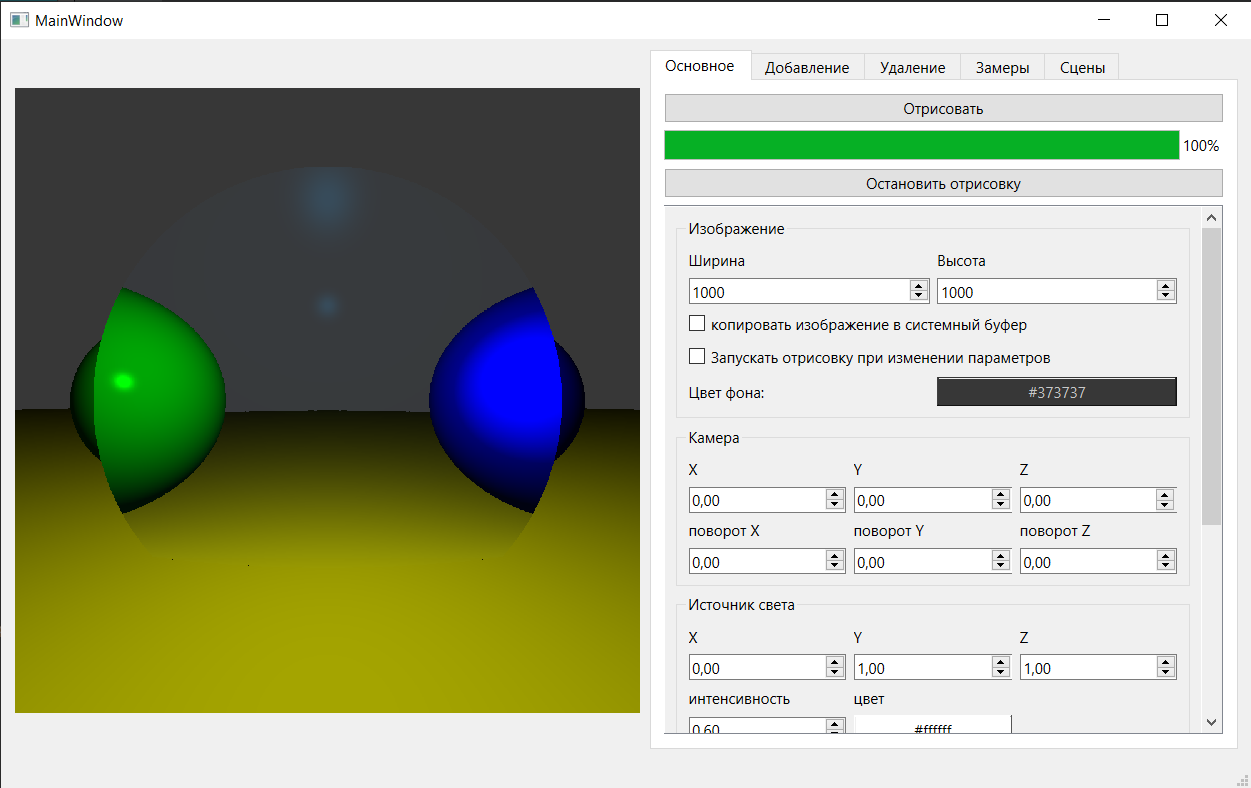
\includegraphics[scale=0.6]{inc/img/ui.png}
	\caption{Интерфейс программы}
	\label{img:ui}
\end{figure}

\clearpage

\subsection*{Вывод}
В данном разделе были выбраны средства реализации, описана схема классов, реализованы выбранные алгоритмы и разработано программное обеспечение.
\clearpage

